\documentclass[11pt]{article}
\usepackage[top = 0.6 in, bottom = 0.6 in, left = 1 in, right = 1 in]{geometry}
\usepackage{graphicx}
% \usepackage{caption2}
% \usepackage{anyfontsize}
\usepackage{setspace}
\usepackage{listings}
\usepackage{xcolor}
\usepackage{float}
\usepackage{amsmath}
\usepackage{subcaption}
\usepackage{lineno}
\usepackage{fancyhdr}

%\usepackage{mwe}
\setlength{\parindent}{0em}
\setlength{\parskip}{1em}
\renewcommand{\baselinestretch}{1.5}

\title{Predicting Academic Funding Success Using Machine Learning Approach}
\author{Jingkai Sun (CID: 01991822)}
\date{\today}


\begin{document}


\begin{titlepage}

    \newcommand{\HRule}{\rule{\linewidth}{0.5mm}} % Defines a new command for the horizontal lines, change thickness here
    % \newcommand{\wordcount}{\input{TPC_project.sum}} % Supervisor's Name

    %----------------------------------------------------------------------------------------
    %	LOGO SECTION
    %----------------------------------------------------------------------------------------

    
\includegraphics[width=7cm]{img/logo.eps}\\[1cm]
    % Include a department/university logo - this will require the graphicx package

    %----------------------------------------------------------------------------------------

    \center % Center everything on the page

    %----------------------------------------------------------------------------------------
    %	HEADING SECTIONS
    %----------------------------------------------------------------------------------------

    % \textsc{\LARGE MSc Computational Methods in Ecology and Evolution}\\[1.5cm] % Name of your university/college
    \textbf{\large Imperial College London}\\[0.8 cm] % Major heading such as course name
    \textbf{\large Department of Life Sciences, Faculty of Natural Sciences}\\[0.8 cm] % Minor heading such as course title
    %----------------------------------------------------------------------------------------
    %	TITLE SECTION
    %----------------------------------------------------------------------------------------
    \makeatletter
    \HRule \\[0.6cm]
    { \huge \bfseries \@title}\\[0.6cm] % Title of your document
    \HRule \\[1.5cm]

    \begin{minipage}{0.4\textwidth}
      \begin{flushleft} \large
      \emph{\textbf{Author:}}\\
      Jingkai \textsc{SUN} \\[0.5cm]
      \emph{\textbf{CID:}}\\
      01991822
      \end{flushleft}
      \end{minipage}
      ~
    \begin{minipage}{0.5\textwidth}
      \begin{flushright} \large
      \emph{\textbf{Supervisors:}} \\
      Dr. David Orme \\
      Dr. James Rosindell \\
      Dr. Samraat Pawar \\

      \emph{\textbf{Email:}} \\
      ks3020@ic.ac.uk
      % \wordcount
      \end{flushright}
    \end{minipage}\\[1cm]

    \vspace*{0.5cm}
    \today \\ % Date


    % \center
    % \textbf{\huge Word Count: 2065}

    \vfill % Fill the rest of the page with whitespace

    \end{titlepage}


% Creating a fancy header
%---------------------------------
\pagestyle{fancy}
\fancyhf{}
\rhead{CID: 01991822}
\lhead{Jingkai Sun}
\rfoot{Page \thepage}
%----------------------------------

% \maketitle
\linenumbers

\section*{Keywords}
Machine Learning (ML), Text Mining, Biology, Natural Language Processing (NLP), Scientific Funding Success, Quantitative Methods, Statistical Analysis


\section{Introduction and Project Ideas}

Academic funding provides essential support for scientists. With an increase in the number of researchers and scientists all over the world, the competition of the academic job market is increasingly fierce, so that the probability of funding success is decreasing. Hence, it is important to understand what determines funding success and how it will be biased due to different reasons.

So far, numerous quantitative measures in the performance of researchers had been proposed \cite{Scientific_success}, such as h-index \cite{Hirsch16569} and impact factor \cite{VANDIJK2014R516}. Also, due to the development of big data and machine learning, many researchers started to study determinants of scientific success using statistical and machine learning methods\cite{Future_impact}\cite{Scientific_success}\cite{VANDIJK2014R516}. However, no research has been done for studying the potential key factors and prediction on funding success using such quantitative methods. Therefore, the object of this project is to study the determinants of funding success. The relevant questions are:
\begin{itemize}
    \item What are the most influential factors to determine the probability of funding success in biological science?
    \item How do these factors affect the funding success?
    \item Are funding success predictable using the Machine Learning approach?
    \item Are predicted outcomes robust in other subject areas?
    \item Do phrases in the paper improve the accuracy of the predicted outcomes? (to be discussed if time is available)
\end{itemize}

\section{Proposed Methods}

All text data, split into training and test datasets, will be obtained from the database of UKRI, NSF, NIH and ERC. I plan to extract features from text data and build a statistical model in training sets to find the key factors of which weights of the model are statistically significant. i.e. I will analyse all funded papers and find the common factors among them, then using a statistical model to see whether they are statistically siginificant. Then these features will be used to fit different machine learning models. Afterwards, I will use the best-fitted model to predict testing sets. Also, if time is available, I plan to use the NLP method to analyse the phrases in the funded paper and to see if the phrases have strong predictive power.


\section{Anticipated Outcomes}

In this project, I assume there are lots of factors determining the funding success. Thus, after analysis, many factors that have a siginificant effect to funding success should be found, so that I can use them to make predictions. Also, phrases have been proved to have strongly predictive power on Kickstarter, which is a website on which entrepreneurs look for funding \cite{inproceedings}. Hence, I assume that phrases will also boost predicted accuracy on my research purpose, which is another outcome I expect to obtain.

\section{Timeline and Feasibility}

\begin{figure}[H]
    \centering
    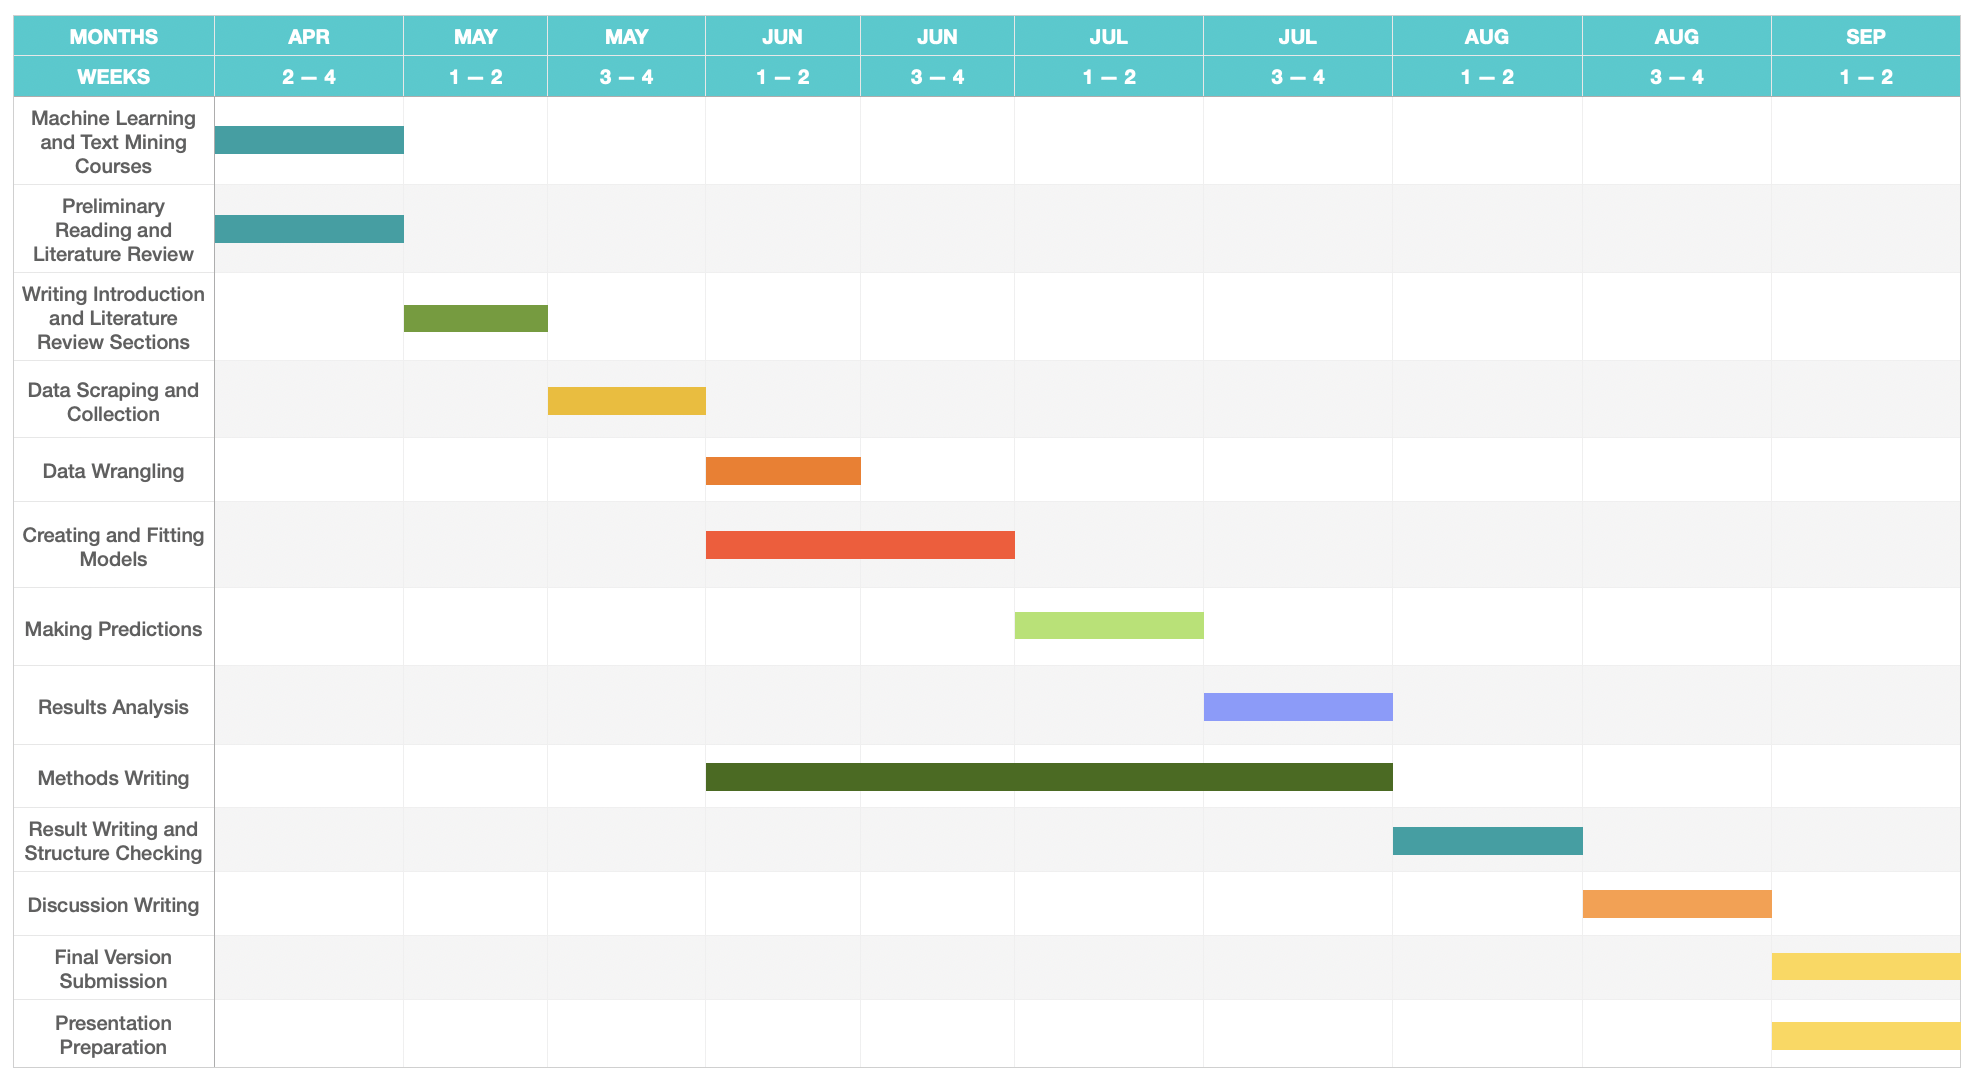
\includegraphics[width = 18cm, height = 10cm]{img/timeline.png}
    \caption{Project Timeline}
\end{figure}

\section{Budget}

None

\bibliographystyle{plain}
\bibliography{../Citation/references}


% \section{Appendices}
\end{document}
